\documentclass[crop,tikz]{standalone}
\usetikzlibrary{backgrounds}
\colorlet{blue}{cyan}
\tikzset{
  inverted/.style = {
    color=white,
    background rectangle/.style={fill},
    show background rectangle
  }
}

\usepackage{amsmath,amssymb}
\usepackage{physics}
\usepackage{pgfplots}
\pgfplotsset{compat=1.16}
\tikzset{>=latex}

\pgfplotsset{
  inverted/.style = {
    every axis legend/.append style={
      draw=white,
      fill=white,
      text=white
    }
  }
}

\begin{document}
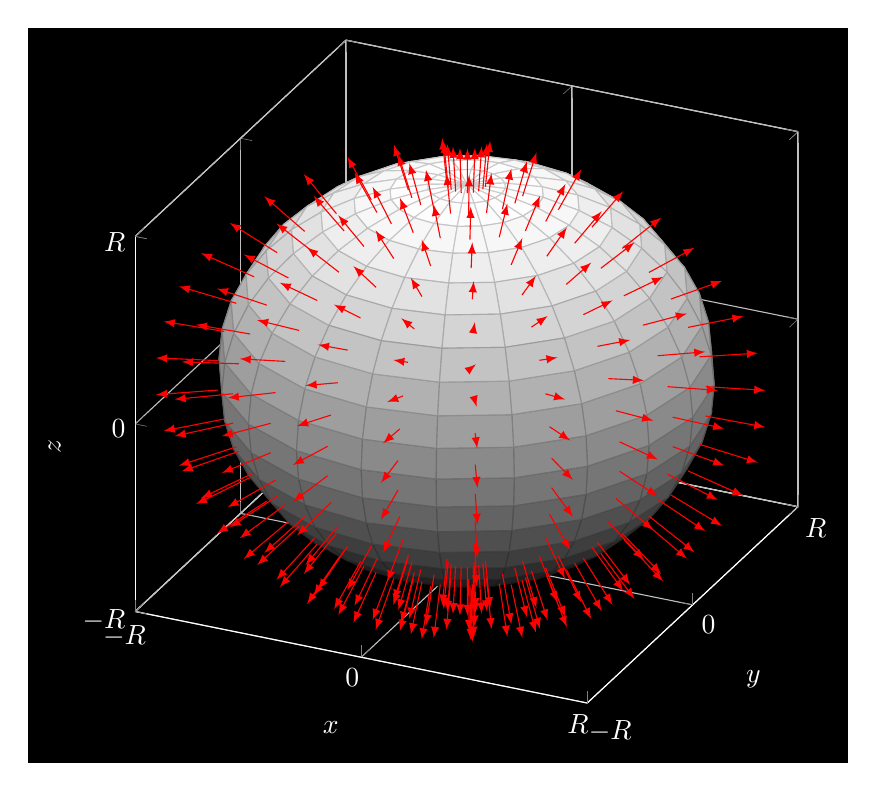
\begin{tikzpicture}[inverted,inverted]
  \pgfmathsetmacro{\nphi}{20}
  \pgfmathsetmacro{\nz}{20}
  \begin{axis}[inverted,
    width=10cm,
    height=10cm,
    xlabel={$x$}, ylabel={$y$}, zlabel={$z$},
    xmin=-1,xmax=1,
    ymin=-1,ymax=1,
    zmin=-1,zmax=1,
    xtick={-1,0,1},
    xticklabels={$-R$,$0$,$R$},
    ytick={-1,0,1},
    yticklabels={$-R$,$0$,$R$},
    ztick={-1,0,1},
    zticklabels={$-R$,$0$,$R$},
    grid,
    samples={\nz+1}, samples y={\nz+1},
    z buffer=sort,
    ]
    \addplot3[
      surf,
      colormap/blackwhite,
      domain=0:{2*pi},
      domain y=0:{pi}
    ] ({cos(deg(x))*sin(deg(y))},{sin(deg(x))*sin(deg(y))},{cos(deg(y))});
    \addplot3[red,
      quiver = {
        u = {x},
        v = {y},
        w = {z},
        scale arrows = 0.25,
        every arrow/.append style={-latex},
      },
      samples={\nphi/2}, samples y={\nz},
      domain={-pi + 2*pi/\nphi + pi/\nphi}:{2*pi/\nphi - pi/\nphi},
      domain y={pi/(2*\nphi)}:{pi - pi/(2*\nphi)},
    ] ({cos(deg(x))*sin(deg(y))},{sin(deg(x))*sin(deg(y))},{cos(deg(y))});
  \end{axis}
\end{tikzpicture}
\end{document}
